\subsection{\texorpdfstring{\nitrogen{}}{15N} sensitivity-enhanced HSQC}
\label{subsec:noah__sehsqc_n}

The implementation of the \nitrogen{} seHSQC modules is entirely identical to the \carbon{} versions previously discussed (\cref{subsec:noah__sehsqc_c}), except for the following points:
\begin{itemize}
    \item CTP gradient amplitudes were set using $g_1 = 80\%$ and $g_2 = \mp 16.2\%$ (note the sign change because of the negative magnetogyric ratio of \nitrogen);
    \item CTP gradient durations were lengthened to \qty{2.5}{\ms} (as discussed for the \nitrogen{} HMQC) in order to suppress artefacts in the seHSQC itself;
    \item the delays $\Delta$ and $\Delta'$ were both set to $1/(4 \cdot \oneJ{NH})$ to maximise sensitivity for \ch{NH} groups;
    \item \carbon{} adiabatic pulses were replaced with hard pulses on \nitrogen{}.
\end{itemize}

Multiplicity editing was not implemented or used in the \nitrogen{} experiments; there is generally little need for this.

\subsubsection{Sensitivity analysis}

The seHSQC is expected to provide sensitivity gains over the HMQC for two reasons: first, the seHSQC peaks are not split by $\nJ{HH}$ in the indirect dimension, and secondly, the PEP transfer element leads to (in theory) a doubling in sensitivity for \ch{NH} groups.
To quantify these gains, I ran several \noah{X,Sp,Cc} experiments, where the first module was a \nitrogen{} HSQC, seHSQC1, or seHSQC2 module (\cref{fig:n15_sens}).
Including the \nitrogen{} HSQC module in this analysis allows us to determine how much of the sensitivity gain is due to multiplet collapse, and how much is due to the sensitivity enhancement block.
The peak at \qty{8.0}{\ppm} is folded and is therefore omitted from this analysis.

\begin{figure}[!ht]
    \centering
    \includegraphics[]{noah/n15_modules_sens.png}%
    {\phantomsubcaption\label{fig:n15_sens_hsqc}}%
    {\phantomsubcaption\label{fig:n15_sens_hsqcp}}%
    {\phantomsubcaption\label{fig:n15_sens_sehsqc1}}%
    {\phantomsubcaption\label{fig:n15_sens_sehsqc1p}}%
    {\phantomsubcaption\label{fig:n15_sens_sehsqc2}}%
    {\phantomsubcaption\label{fig:n15_sens_sehsqc2p}}%
    \caption[Comparison of sensitivities of NOAH \nitrogen{} modules]{
        Comparison of NOAH \proton{}--\nitrogen{} modules; the 2D spectra and their positive projections onto the $F_1$ axis are shown.
        Numbers above each peak in the projections indicate sensitivity increases compared to the HMQC module (see, e.g., \cref{fig:hmqc_scale_std2,fig:hmqc_scale_std1}).
        \textbf{(\subref*{fig:n15_sens_hsqc})--(\subref*{fig:n15_sens_hsqcp})} HSQC module.
        \textbf{(\subref*{fig:n15_sens_sehsqc1})--(\subref*{fig:n15_sens_sehsqc1p})} seHSQC1 module.
        \textbf{(\subref*{fig:n15_sens_sehsqc2})--(\subref*{fig:n15_sens_sehsqc2p})} seHSQC2 module.
        \datacode{7G-201017}
    }
    \label{fig:n15_sens}
\end{figure}

As can be seen, the HSQC alone allows for substantial sensitivity increases over the HMQC, with over $3\times$ gains being accomplished simply due to multiplet collapse.
The seHSQC experiments push this even further, with an approximate $1.5\times$ sensitivity improvement for all peaks.
In contrast to the \carbon{} case, the \nitrogen{} seHSQC1 module outperforms seHSQC2 in terms of raw sensitivity, though (as before) there is no clear explanation for this subtle difference.

\begin{figure}[!ht]
    \centering
    \includegraphics[]{noah/n15_later_modules_sens.png}%
    {\phantomsubcaption\label{fig:n15_later_sens_hsqc}}%
    {\phantomsubcaption\label{fig:n15_later_sens_hsqcp}}%
    {\phantomsubcaption\label{fig:n15_later_sens_hsqcplot}}%
    {\phantomsubcaption\label{fig:n15_later_sens_sehsqc1}}%
    {\phantomsubcaption\label{fig:n15_later_sens_sehsqc1p}}%
    {\phantomsubcaption\label{fig:n15_later_sens_sehsqc1plot}}%
    {\phantomsubcaption\label{fig:n15_later_sens_sehsqc2}}%
    {\phantomsubcaption\label{fig:n15_later_sens_sehsqc2p}}%
    {\phantomsubcaption\label{fig:n15_later_sens_sehsqc2plot}}%
    \caption[Comparison of \carbon{} seHSQC sensitivity when preceded by different \nitrogen{} modules]{
        Comparison of the \carbon{} seHSQC module from \noah{X,Sp,Cc} supersequences, where X is a \proton{}--\nitrogen{} module.
        The 2D spectra, their positive projections onto the $F_1$ axis, as well as the relative intensities of all peaks (as compared to the corresponding module in the \noah{Mn,Sp,Cc} supersequence), are shown.
        \textbf{(\subref*{fig:n15_later_sens_hsqc})--(\subref*{fig:n15_later_sens_hsqcplot})} X = \nitrogen{} HSQC.
        \textbf{(\subref*{fig:n15_later_sens_sehsqc1})--(\subref*{fig:n15_later_sens_sehsqc1plot})} X = \nitrogen{} seHSQC1.
        \textbf{(\subref*{fig:n15_later_sens_sehsqc2})--(\subref*{fig:n15_later_sens_sehsqc2plot})} X = \nitrogen{} seHSQC2.
        \datacode{7G-201017}
    }
    \label{fig:n15_later_sens}
\end{figure}

However, this apparent advantage of the seHSQC1 vanishes when looking at the \carbon{} seHSQC module which comes later in the supersequence.
When preceded by the \nitrogen{} HSQC or seHSQC1 modules, this module suffers from severely decreased sensitivity (\cref{fig:n15_later_sens}) as compared to when the seHSQC2 module is used.
As the spectra and their $F_1$ projections show, this reduction in sensitivity actually stems from broadening in the indirect dimension.
This in turn arises because \magnnot{N} magnetisation (which includes the \magn{C} component sampled in this module) precesses in the transverse plane during the $t_1$ period of the \nitrogen{} HSQC and seHSQC1.
Evolution of $\nJ{HH}$, as well as $T_2$ relaxation, lead to a $t_1$-dependent signal loss which (after Fourier transformation) is manifested as line broadening and ca.\ 65\% decreased peak heights (\cref{fig:n15_later_sens_hsqcplot,fig:n15_later_sens_sehsqc1plot}).

While the \nitrogen{} seHSQC2 module also does not preserve \magnnot{N} magnetisation as well as the HMQC module (with an approximately 20\% loss, see \cref{fig:n15_later_sens_sehsqc2plot}), this is not anywhere as drastic as with the other modules.
Furthermore, these losses are constant across all $t_1$ increments, so there is no line broadening observed in the modules which follow.
This small sensitivity loss in later modules is also a reasonable price to pay for the improvement in the \nitrogen{} module itself: typically, it is the \nitrogen{} module which has the smallest intrinsic sensitivity, so it is desirable to maximise this.

It should be noted that the \carbon{} seHSQC1 (and HSQC) modules also do place \magnnot{C} magnetisation in the transverse plane during $t_1$.
However, they do not cause (appreciable) broadening in downstream modules, as evidenced by the almost complete preservation of CLIP-COSY peak heights in \cref{fig:noah_sehsqc_comp}.
This is because indirect-dimension spectral windows for \carbon{} experiments are often much wider, and the acquisition times ($\AQ$, following on from \cref{subsec:noah__hmqc}) consequently shorter.
For example, in the \noah{X,Sp,Cc} experiments shown here, the values of $\AQ$ for the \nitrogen{} and \carbon{} experiments are respectively \qty{60.1}{\ms} and \qty{5.38}{\ms}.


\subsubsection{CTP gradient duration}

To verify that the \qty{2.5}{\ms} CTP gradients were necessarily in the \nitrogen{} seHSQC as well, I repeated the \noah{Spn,Sp,Cc} experiment with increasing gradient durations.
Only the seHSQC2 module was studied.
It should be noted that the durations of \textit{only} the CTP gradients $g_1$ and $g_2$ (in \cref{fig:sehsqc_po_noah2}) were modified; $g_3$ and $g_4$ retain their original durations of \qty{1}{\ms}.
The results, shown in \cref{fig:sehsqc_cnst16}, are qualitatively very similar to that obtained with the HMQC (in \cref{fig:hmqc_cnst16}): increasing the gradient duration does not lead to substantial differences in signal intensity, but does provide much improved artefact suppression.
In this case, equivalent results can be obtained using gradient durations of \qtyrange{2.2}{2.3}{\ms}; however, \qty{2.5}{\ms} still appears to be a reliable `default' value which can be used without further optimisation.

\begin{figure}[!ht]
    \centering
    \includegraphics[]{noah/sehsqc_cnst16_scan.png}%
    \caption[Variation of seHSQC2 signal and artefact intensity with CTP gradient duration]{
        Variation of seHSQC2 signal and artefact intensity with CTP gradient duration, as measured by (absolute) peak heights in the positive $F_2$ projection.
        \datacode{7Z-200926}
    }
    \label{fig:sehsqc_cnst16}
\end{figure}


\subsubsection{$k$- and SW-scaling}

Finally, the effects of $k$- and SW-scaling were also investigated for the seHSQC2 module.
The effects of just performing scaling are very minimal (\cref{fig:sehsqc_scale}): unlike the HMQC module where lowering the resolution avoids losses in peak height due to multiplet structure, there are no such gains for the seHSQC module.
The use of indirect-dimension linear prediction, however, is rather more successful for the seHSQC module (\cref{fig:sehsqc_scale_lp}): again this likely stems from the lack of multiplet structure in $F_1$.
As before, the application of LP to the SW-scaled spectra yields better peak shapes than the $k$-scaled spectra (compare, e.g., \cref{fig:sehsqc_scale_lp_k82,fig:sehsqc_scale_lp_sw82}).

\begin{figure}[!htbp]
    \centering
    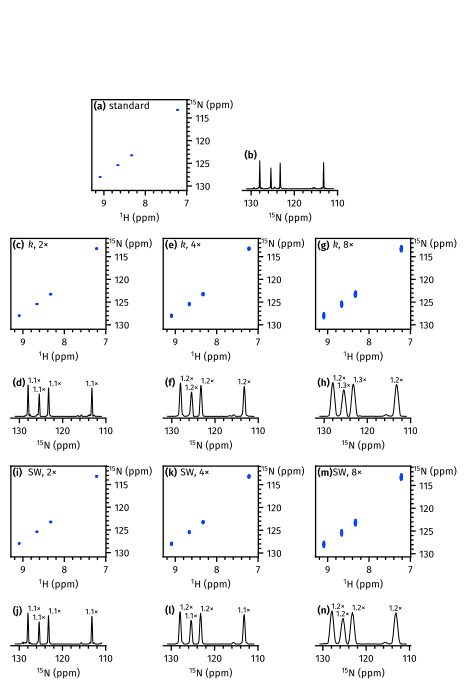
\includegraphics[]{noah/sehsqc_scale.png}%
    {\phantomsubcaption\label{fig:sehsqc_scale_std2}}%
    {\phantomsubcaption\label{fig:sehsqc_scale_std1}}%
    {\phantomsubcaption\label{fig:sehsqc_scale_k22}}%
    {\phantomsubcaption\label{fig:sehsqc_scale_k21}}%
    {\phantomsubcaption\label{fig:sehsqc_scale_k42}}%
    {\phantomsubcaption\label{fig:sehsqc_scale_k41}}%
    {\phantomsubcaption\label{fig:sehsqc_scale_k82}}%
    {\phantomsubcaption\label{fig:sehsqc_scale_k81}}%
    {\phantomsubcaption\label{fig:sehsqc_scale_sw22}}%
    {\phantomsubcaption\label{fig:sehsqc_scale_sw21}}%
    {\phantomsubcaption\label{fig:sehsqc_scale_sw42}}%
    {\phantomsubcaption\label{fig:sehsqc_scale_sw41}}%
    {\phantomsubcaption\label{fig:sehsqc_scale_sw82}}%
    {\phantomsubcaption\label{fig:sehsqc_scale_sw81}}%
    \caption[Effects of $k$- and SW-scaling on NOAH seHSQC2 spectrum]{
        Effects of $k$- and SW-scaling on NOAH seHSQC2 spectrum (taken from \noah{Spn,Sp,Cc} supersequences).
        Each seHSQC spectrum is shown together with a positive projection onto the $F_1$ axis.
        The relative SNR of each peak, with respect to the standard spectrum, is indicated on each of the other projections.
        \textbf{(\subref*{fig:sehsqc_scale_std2})--(\subref*{fig:sehsqc_scale_std1})} Standard spectrum.
        \textbf{(\subref*{fig:sehsqc_scale_k22})--(\subref*{fig:sehsqc_scale_k81})} $k$-scaled spectra.
        \textbf{(\subref*{fig:sehsqc_scale_sw22})--(\subref*{fig:sehsqc_scale_sw81})} SW-scaled spectra.
        \datacode{7G-210310}
    }
    \label{fig:sehsqc_scale}
\end{figure}

\begin{figure}[!htbp]
    \centering
    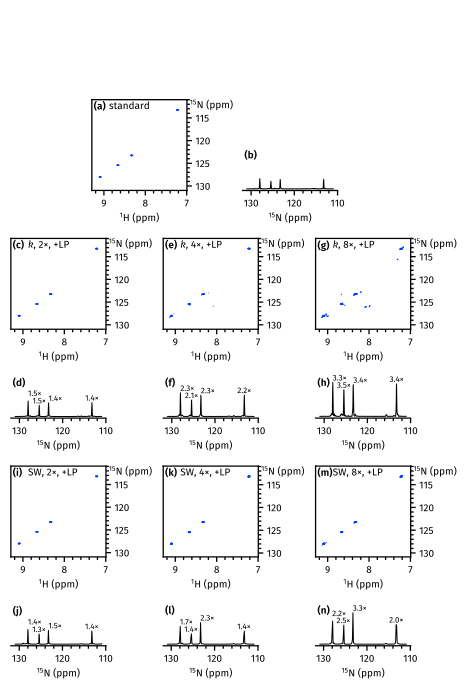
\includegraphics[]{noah/sehsqc_scale_lp.png}%
    {\phantomsubcaption\label{fig:sehsqc_scale_lp_std2}}%
    {\phantomsubcaption\label{fig:sehsqc_scale_lp_std1}}%
    {\phantomsubcaption\label{fig:sehsqc_scale_lp_k22}}%
    {\phantomsubcaption\label{fig:sehsqc_scale_lp_k21}}%
    {\phantomsubcaption\label{fig:sehsqc_scale_lp_k42}}%
    {\phantomsubcaption\label{fig:sehsqc_scale_lp_k41}}%
    {\phantomsubcaption\label{fig:sehsqc_scale_lp_k82}}%
    {\phantomsubcaption\label{fig:sehsqc_scale_lp_k81}}%
    {\phantomsubcaption\label{fig:sehsqc_scale_lp_sw22}}%
    {\phantomsubcaption\label{fig:sehsqc_scale_lp_sw21}}%
    {\phantomsubcaption\label{fig:sehsqc_scale_lp_sw42}}%
    {\phantomsubcaption\label{fig:sehsqc_scale_lp_sw41}}%
    {\phantomsubcaption\label{fig:sehsqc_scale_lp_sw82}}%
    {\phantomsubcaption\label{fig:sehsqc_scale_lp_sw81}}%
    \caption[Effects of $k$- and SW-scaling on NOAH seHSQC2 spectrum with extra linear prediction]{
        The same as in \cref{fig:sehsqc_scale}, but with extra linear prediction applied to all scaled spectra to bring $\AQeff$ up to its original value in the standard spectrum.
        Linear prediction of $k$ times more points leads to a $\sqrt{k}$ increase in noise; to account for this, all spectra are plotted with the same noise level.
        \textbf{(\subref*{fig:sehsqc_scale_lp_std2})--(\subref*{fig:sehsqc_scale_lp_std1})} Standard spectrum.
        \textbf{(\subref*{fig:sehsqc_scale_lp_k22})--(\subref*{fig:sehsqc_scale_lp_k81})} $k$-scaled spectra.
        \textbf{(\subref*{fig:sehsqc_scale_lp_sw22})--(\subref*{fig:sehsqc_scale_lp_sw81})} SW-scaled spectra.
        \datacode{7G-210310}
    }
    \label{fig:sehsqc_scale_lp}
\end{figure}
